\chapter{Pendahuluan}
\chapterauthor{Alfa Yohannis, Charlie Chaplin}

\documentclass{article}
\usepackage{indentfirst}
\setlength{\parskip}{20pt}
\usepackage[utf8]{inputenc}
\usepackage{graphicx}
\graphicspath{{images/}}
\usepackage{varwidth}

\begin{document}
	\begin{titlepage}
		\begin{center}
			\textbf{\huge Orchestration-driven Service-oriented Architecture}
			
			\vspace{0.5cm}
				
			{\large Software Architecture}
			
			\vspace{2.5cm}
			
			\section*{Nama}
			\begin{varwidth}{\textwidth}
				\begin{itemize}
					\item Yefta Tanuwijaya 2110101032
					\item Hansel Ricardo 2110101020
					\item Jonathan Erik Maruli Tua 2110101026
				\end{itemize}
			\end{varwidth}

			
			
		\end{center}

	\end{titlepage}
	\section{Definisi}
	Orchestration-driven Service-oriented Architecture (ODSOA) adalah suatu pendekatan arsitektur perangkat lunak yang bertujuan untuk memfasilitasi pengembangan dan integrasi sistem yang kompleks dengan cara menggunakan layanan (services) yang terdistribusi dan 		terpisah secara fisik namun saling terkait secara fungsional.

	ODSOA menempatkan Orkestrasi (Orchestration) sebagai elemen kunci untuk mengelola interaksi antara layanan. Orkestrasi dapat didefinisikan sebagai proses otomatis yang mengkoordinasikan dan mengatur eksekusi layanan secara teratur untuk mencapai tujuan bisnis 		tertentu.

	Dalam ODSOA, layanan disediakan sebagai fungsi-fungsi modular yang dapat digunakan oleh aplikasi dan sistem lain untuk memperoleh fungsionalitas tambahan. Layanan ini biasanya disediakan secara independen oleh unit bisnis atau departemen yang berbeda dan dapat 	diakses melalui jaringan.

	ODSOA memiliki beberapa keuntungan, antara lain: skalabilitas, fleksibilitas, dan interoperabilitas. Skalabilitas memungkinkan sistem untuk diukur dan meningkatkan kapasitasnya dengan mudah. Fleksibilitas memungkinkan pengguna untuk menyesuaikan layanan sesuai 		kebutuhan mereka tanpa harus mengubah keseluruhan arsitektur. Interoperabilitas memungkinkan sistem untuk berinteraksi dengan sistem lain yang menggunakan standar yang sama.

	Secara keseluruhan, ODSOA dapat membantu perusahaan dalam mempercepat pengembangan dan integrasi aplikasi serta meningkatkan efisiensi dan efektivitas bisnis secara keseluruhan.
	
	\section{Orchestration-driven Service-oriented Architecture Schema
	}
	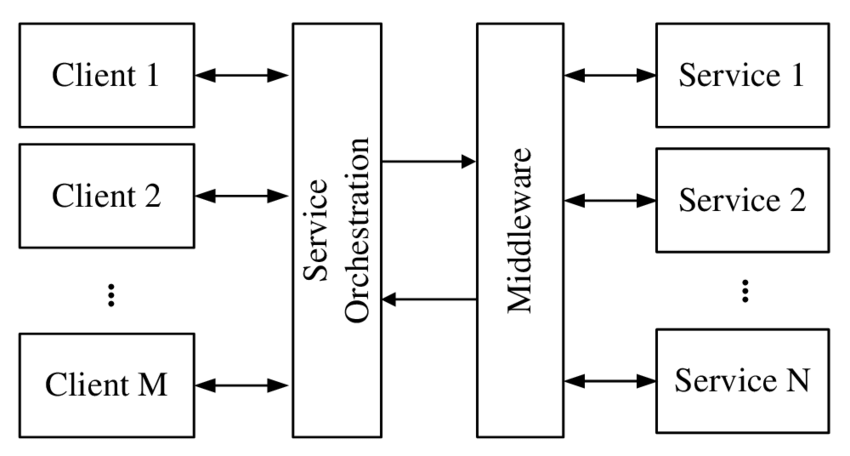
\includegraphics[scale=0.4]{images/ODSOA.png}
	Orchestration-driven Service-oriented Architecture (ODSOA) Schema adalah suatu model yang menggambarkan arsitektur ODSOA secara visual, yang mencakup komponen-komponen utama dan interaksi antara mereka. Beberapa komponen utama dalam schema ODSOA 		antara lain:
\begin{itemize}
	\item Layanan (Services): Komponen inti dari ODSOA adalah layanan, yang merupakan unit fungsional yang terdistribusi secara terpisah namun saling terkait secara fungsional. Layanan ini dapat digunakan oleh aplikasi dan sistem lain untuk memperoleh fungsionalitas 				tambahan.

	\item Orkestrasi (Orchestration): Orkestrasi merupakan proses otomatis yang mengkoordinasikan dan mengatur eksekusi layanan secara teratur untuk mencapai tujuan bisnis tertentu. Orkestrasi dapat mengatur urutan dan kondisi yang harus dipenuhi oleh layanan.

	\item Bus Layanan (Service Bus): Bus Layanan adalah infrastruktur yang memfasilitasi komunikasi antara layanan dalam arsitektur ODSOA. Bus Layanan dapat mengatur dan mengarahkan permintaan dan respons antara layanan.

	\item Repositori Layanan (Service Repository): Repositori Layanan adalah tempat untuk menyimpan informasi terkait dengan layanan yang tersedia, seperti deskripsi, spesifikasi teknis, dan interdependensi antara layanan. Repositori Layanan memungkinkan pengguna 			untuk mencari dan menemukan layanan yang dibutuhkan.

	\item Klien (Client): Klien adalah aplikasi atau sistem yang menggunakan layanan untuk memperoleh fungsionalitas tambahan. Klien mengirim permintaan ke layanan dan menerima respons dari layanan.

	\item Penyedia Layanan (Service Provider): Penyedia Layanan adalah unit bisnis atau departemen yang menyediakan layanan untuk digunakan oleh aplikasi dan sistem lain. Penyedia Layanan bertanggung jawab untuk mengembangkan dan menjaga layanan yang 			disediakan.
\end{itemize}

	Dalam ODSOA Schema, interaksi antara komponen-komponen tersebut direpresentasikan dengan panah yang menghubungkan mereka. Misalnya, panah dari klien ke layanan menunjukkan bahwa klien menggunakan layanan tersebut, sedangkan panah dari layanan ke bus 		layanan menunjukkan bahwa layanan terdaftar dalam infrastruktur bus layanan. Dengan ODSOA Schema, pengguna dapat dengan mudah memahami arsitektur ODSOA secara visual dan mengidentifikasi komponen-komponen utama dan interaksi antara mereka.

	\section{Kelebihan}
	
	\begin{itemize}
		\item Skalabilitas: ODSOA memungkinkan sistem untuk diukur dan meningkatkan kapasitasnya dengan mudah. Layanan dapat dikonfigurasi ulang atau ditambahkan ke infrastruktur dengan mudah, tanpa mempengaruhi sistem keseluruhan. Hal ini memudahkan 					perusahaan untuk menyesuaikan sistem mereka dengan perubahan kebutuhan bisnis.
		\item Fleksibilitas: ODSOA memungkinkan pengguna untuk menyesuaikan layanan sesuai kebutuhan mereka tanpa harus mengubah keseluruhan arsitektur. Dengan demikian, perusahaan dapat dengan mudah memodifikasi fungsionalitas sistem dan mengintegrasikan 				solusi baru tanpa mempengaruhi sistem keseluruhan.
		\item Interoperabilitas: ODSOA memungkinkan sistem untuk berinteraksi dengan sistem lain yang menggunakan standar yang sama. Hal ini memungkinkan perusahaan untuk berintegrasi dengan sistem lain dengan mudah dan memperluas fungsionalitas sistem 					mereka.
		\item Reusabilitas: Layanan dalam ODSOA adalah modular dan dapat digunakan kembali oleh aplikasi dan sistem lain. Hal ini memungkinkan perusahaan untuk mengembangkan sistem dengan cepat dan efisien.
		\item Pemisahan Tugas: ODSOA memisahkan tugas-tugas sistem menjadi layanan yang terpisah secara fisik namun saling terkait secara fungsional. Hal ini memudahkan manajemen sistem dan memungkinkan perusahaan untuk mengoptimalkan penggunaan sumber 				daya.
	\end{itemize}
.
	
	
	\section{Kekurangan}
	
	\begin{itemize}
		\item Kompleksitas: Arsitektur ODSOA dapat menjadi sangat kompleks, terutama ketika menangani banyak layanan yang berbeda dan memerlukan integrasi yang kompleks. Oleh karena itu, perusahaan memerlukan tingkat keahlian teknis yang tinggi untuk 					mengimplementasikan dan mengelola arsitektur ini dengan efektif.
		\item Keamanan: Arsitektur ODSOA dapat menimbulkan masalah keamanan karena penggunaannya yang melibatkan layanan dari banyak sistem dan vendor. Oleh karena itu, perusahaan harus memperhatikan masalah keamanan yang terkait dengan integrasi dan 				melakukan tindakan yang tepat untuk mengurangi risiko keamanan.
		\item Pengelolaan versi: Dalam ODSOA, perubahan pada satu layanan dapat mempengaruhi layanan lainnya. Oleh karena itu, pengelolaan versi menjadi penting untuk memastikan bahwa perubahan yang dibuat pada layanan tidak mengganggu kinerja sistem secara 			keseluruhan.
		\item Biaya: Implementasi arsitektur ODSOA memerlukan biaya yang tinggi karena melibatkan pengembangan, integrasi, dan manajemen layanan yang kompleks. Oleh karena itu, perusahaan harus mempertimbangkan biaya ini sebelum mengimplementasikan 					arsitektur ini.
		\item Ketergantungan terhadap vendor: Terkadang perusahaan tergantung pada vendor tertentu untuk memasok layanan tertentu. Jika vendor tersebut menghentikan layanannya, maka perusahaan perlu mencari alternatif layanan dari vendor lain atau bahkan 				harus mengubah arsitektur sistem secara keseluruhan.
	\end{itemize}

	\section{penerapan dalam aplikasi}

\end{document}

